\documentclass[../_main/handlingar.tex]{subfiles}

\begin{document}
\motion{Utredning om renovering av toaletterna}

Det har knappast undgått någon att toaletterna i Edekvata är i ett uruselt skick. De är både små och med betydande slitage. Långt under standarden för resten av huset och campus. 
Därför tycker jag att det är hög tid för en upprustning här. Ett annat problem sektionen länge haft är vårt begränsade förvaringsutrymme. I princip alla våra förråd är överfulla och trots medlemmars städinsatser förblir de mer eller mindre i kaos. 

Jag har under året som ordförande försökt arbeta fram en lösning på dessa problem och såg en möjlighet i det nu oanvända rummet “Ulla”. Rummet som ligger beläget mellan Caféets lager “CM” och toaletterna har blivit kvar sen tiden sektionen hade en anställd i LED. I rummet finns en toalett och en dusch. Min tanke var att riva detta rum bygga ihop det med “CM” och samtidigt nyttja lite av det frigjorda utrymmet för att renovera toaletterna och göra dem större. Nedan ser ni i den övre bilden hur det ser ut idag och sedan mitt förslag på förändring. 

\begin{center}
    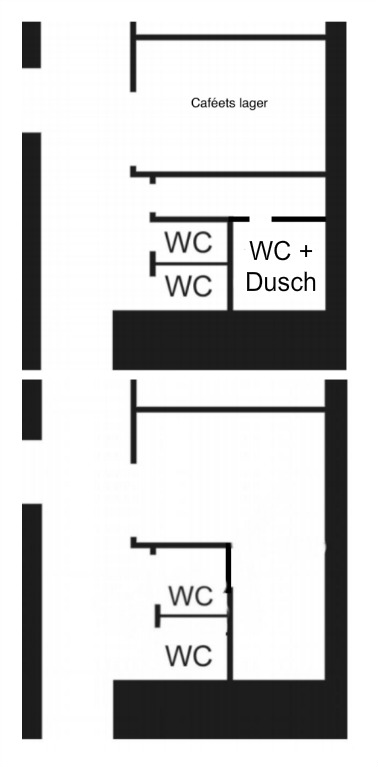
\includegraphics[width=7cm]{toarenov.jpg}
\end{center}

\newpage  
Strax innan sommaren hade vi hantverkare på besök och häromveckan lämnade de en offert på vad renoveringen skulle kosta, 211 000 kr exklusive moms. Dock ska tilläggas att i det förslaget ingick också att anpassa för en tvättmaskin, vilket inte är relevant längre då vi har löst sektionens tvättbehov på annat sätt. 

Hur som helst tar detta förarbete mycket tid och det är inget jag kommer hinna avsluta innan årsskiftet. Därför vill jag söka projektfunktionär för att under det kommande halvåret undersöka detta ytterligare, leta finansiärer och med som mål lägga fram ett förslag till VTM20 för en renovering sommaren 2020.
  
Jag yrkar

\begin{attsatser}
    \att motionären väljs in som projektfunktionär med mandatperiod till Vårterminsmötet 2020, samt 
    \att beslutet läggs på beslutsuppföljningen till VTM/20 med undertecknad som ansvarig.
    
\end{attsatser}

\begin{signatures}{1}
    \isekt
    \signature{Edvard Carlsson}{Ordförande}
\end{signatures}

\end{document}
